\chapter{Simulations}
\label{chap:simulations}

To assess the stabilisation performance after solving the optimisation problem for the bike, some simulations were conducted. The models of the bicycle from Section \ref{sec:bike_modelling} are tested to understand the mathematical behaviour of the bicycle under different controllers.

As stated before, two models of the bicycle were considered:
\begin{itemize}
	\item \textbf{Without Fork Model:} A simplified kinetic model assuming the fork angle is negligible.
	\item \textbf{With Fork Model:} A kinetic model including the fork angle, accounting for the steering head geometry.
\end{itemize}

%\unsure{Not sure about Simulation} Simulation results showed that the \emph{without fork model} generally produced better stabilization performance due to the reduced complexity and linearization assumptions.
%Nevertheless, both models were used to test the robustness and adaptability of the control designs.

%\section{Simulation Setup}
Two versions of the data-driven state-feedback controllers were tested. The first version is a data-driven min-max by solving the SDP in Equation \eqref{eq:final_gamma} only once for an initial state. While the second version is a data-driven min-max MPC where the SDP is solved for each time step. To evaluate the data-driven control laws performance, they are compared to a state-feedback LQR controller.

The simulations were performed using MATLAB based on the kinetic models described in Section~\ref{sec:bike_modelling}.
The following assumptions were made:
\begin{itemize}
	\item The bicycle moves on a horizontal plane.
	\item The rear wheel maintains a constant forward velocity.
	\item Small-angle approximations are applied for the lean angle ($\phi$) and steering angle ($\delta$).
\end{itemize}

The key physical parameters used are summarized in Table~\ref{tab:simulation_parameters}.

\begin{table}[H]
	\centering
	\caption{Simulation Parameters}
	\label{tab:simulation_parameters}
	\begin{tabular}{|c|c|c|p{6cm}|}
		\hline
		\textbf{Parameter} & \textbf{Value} & \textbf{Unit} & \textbf{Description} \\ \hline
		$h$ & 0.088 & m & Height of center of mass \\ \hline
		$b$ & 0.055 & m & Wheelbase \\ \hline
		$\lambda$ & 75 or 90 & degrees & \textbf{Fork angle}: angle between the steering axis and the horizontal line  \\ \hline
		$c$ & 0.087 & m & Trail distance \\ \hline
		$r_w$ & 0.0375 & m & Radius of the wheel \\ \hline
		$r_\tau$ & $r_w \cdot \tan\left(\frac{\pi}{2} - \lambda\right)$ & m & Distance between front wheel ground contract point and intersection of fork with ground \\ \hline
		$g$ & 9.81 & m/s\textsuperscript{2} & Gravitational acceleration \\ \hline
		$v$ & 0.634 & m/s & Forward speed \\ \hline
		$w$ & 0.167 & m & Distance between front and rear wheels at ground contact points \\ \hline

	\end{tabular}
\end{table}

The input and state constraints for the system were defined as follows.
\begin{gather}\nonumber
	S_u = 0.005836, \\
	\nonumber
	S_x =
	\begin{bmatrix}
		2.6798 & 0 & 0 \\
		0 & 0.32828 & 0 \\
		0 & 0 & 2.05
	\end{bmatrix}
\end{gather}

The lean angle is constrained between -40 and 40

The three different simulations corresponding to different control strategies are discussed below.

%\textbf{Linear Quadratic Regulator (LQR)}
\section{Linear Quadratic Regulator (LQR)}
An LQR controller was designed separately for both the fork and no-fork models by solving the discrete-time Algebraic Riccati Equation.
Different weighting matrices $Q$ and $R$ were selected to modify the weights given to the states and inputs respectively, where the weights are used to compute the closed loop cost.

%//(such as $Q = \text{diag}(300, 0, 300)$, $R = 1$ where it gives higher cost to the lean and steering angles and neglects the rate of change of the lean angle. This $R$ does not give a high cost to the input which is the rate of change of the steering angle.)//

The LQR served as a baseline controller and was also tested to generate input-state data necessary for the subsequent data-driven methods.
In \autoref{fig:lqr_sim_figs}, four simulations are conducted to show the difference in performance for different $Q$ and $R$ settings. Matrix $Q$ corresponds to the cost associated with the states, whereas $R$ corresponds to the cost associated with the inputs.
\autoref{fig:lqr4} shows that giving more weight to the second state, namely the lean angle rate of change, smooths the lean angle response and reduces its steepness. Since the input is the steering angle rate of change $\dot{\delta}$, when giving it more weight in \autoref{fig:lqr3} all states are smoothened.

\todo[inline]{I am here now}

\begin{figure}[H]
	\centering
	\begin{subfigure}[b]{0.45\textwidth}
		\centering
		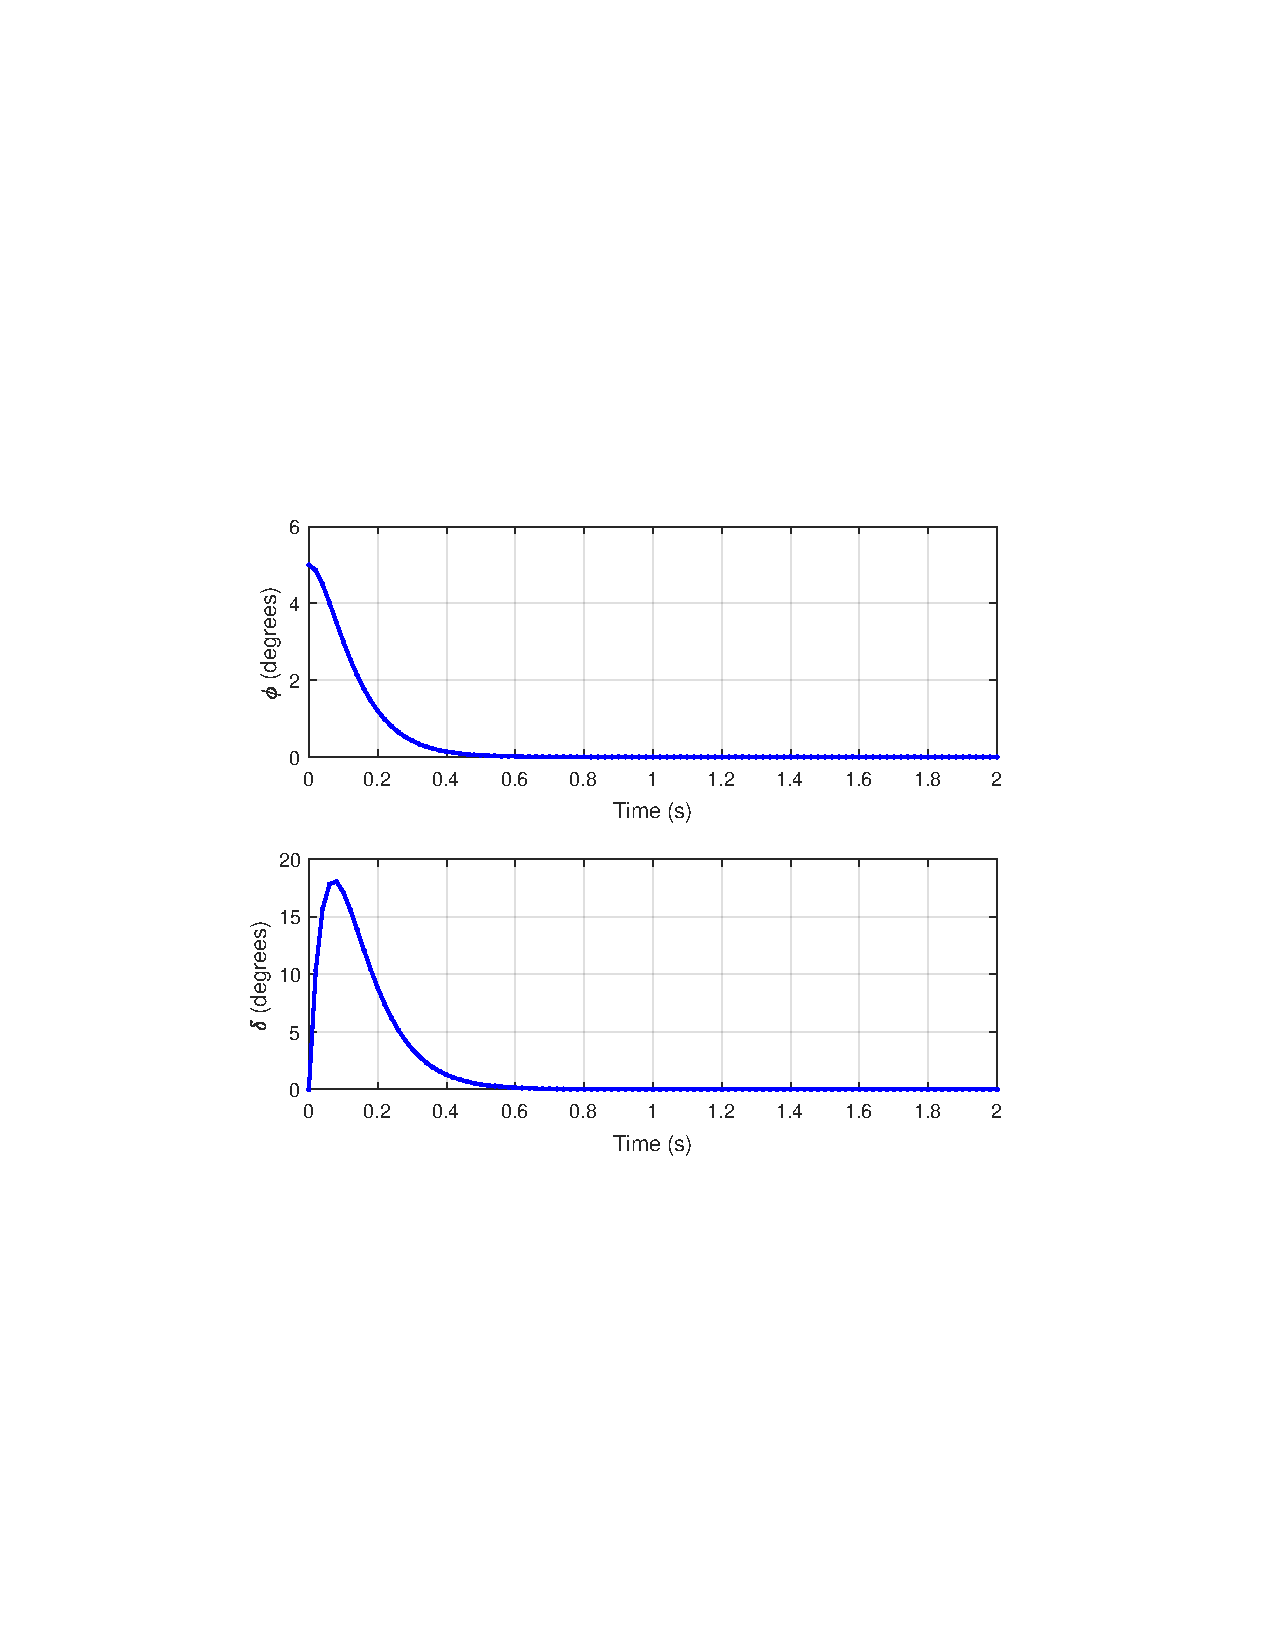
\includegraphics[width=\textwidth, trim=120 240 120 240]{figures/plots/LQR Compute Q(300,0,300)R(1) with 75 fork angle.pdf}
		\caption{\boldmath LQR with $Q = \operatorname{diag}(300,\,0,\,300)$, $R = 1$, $75^\circ$ fork angle.}
		\label{fig:lqr1}
	\end{subfigure}
	\hfill
	\begin{subfigure}[b]{0.45\textwidth}
		\centering
		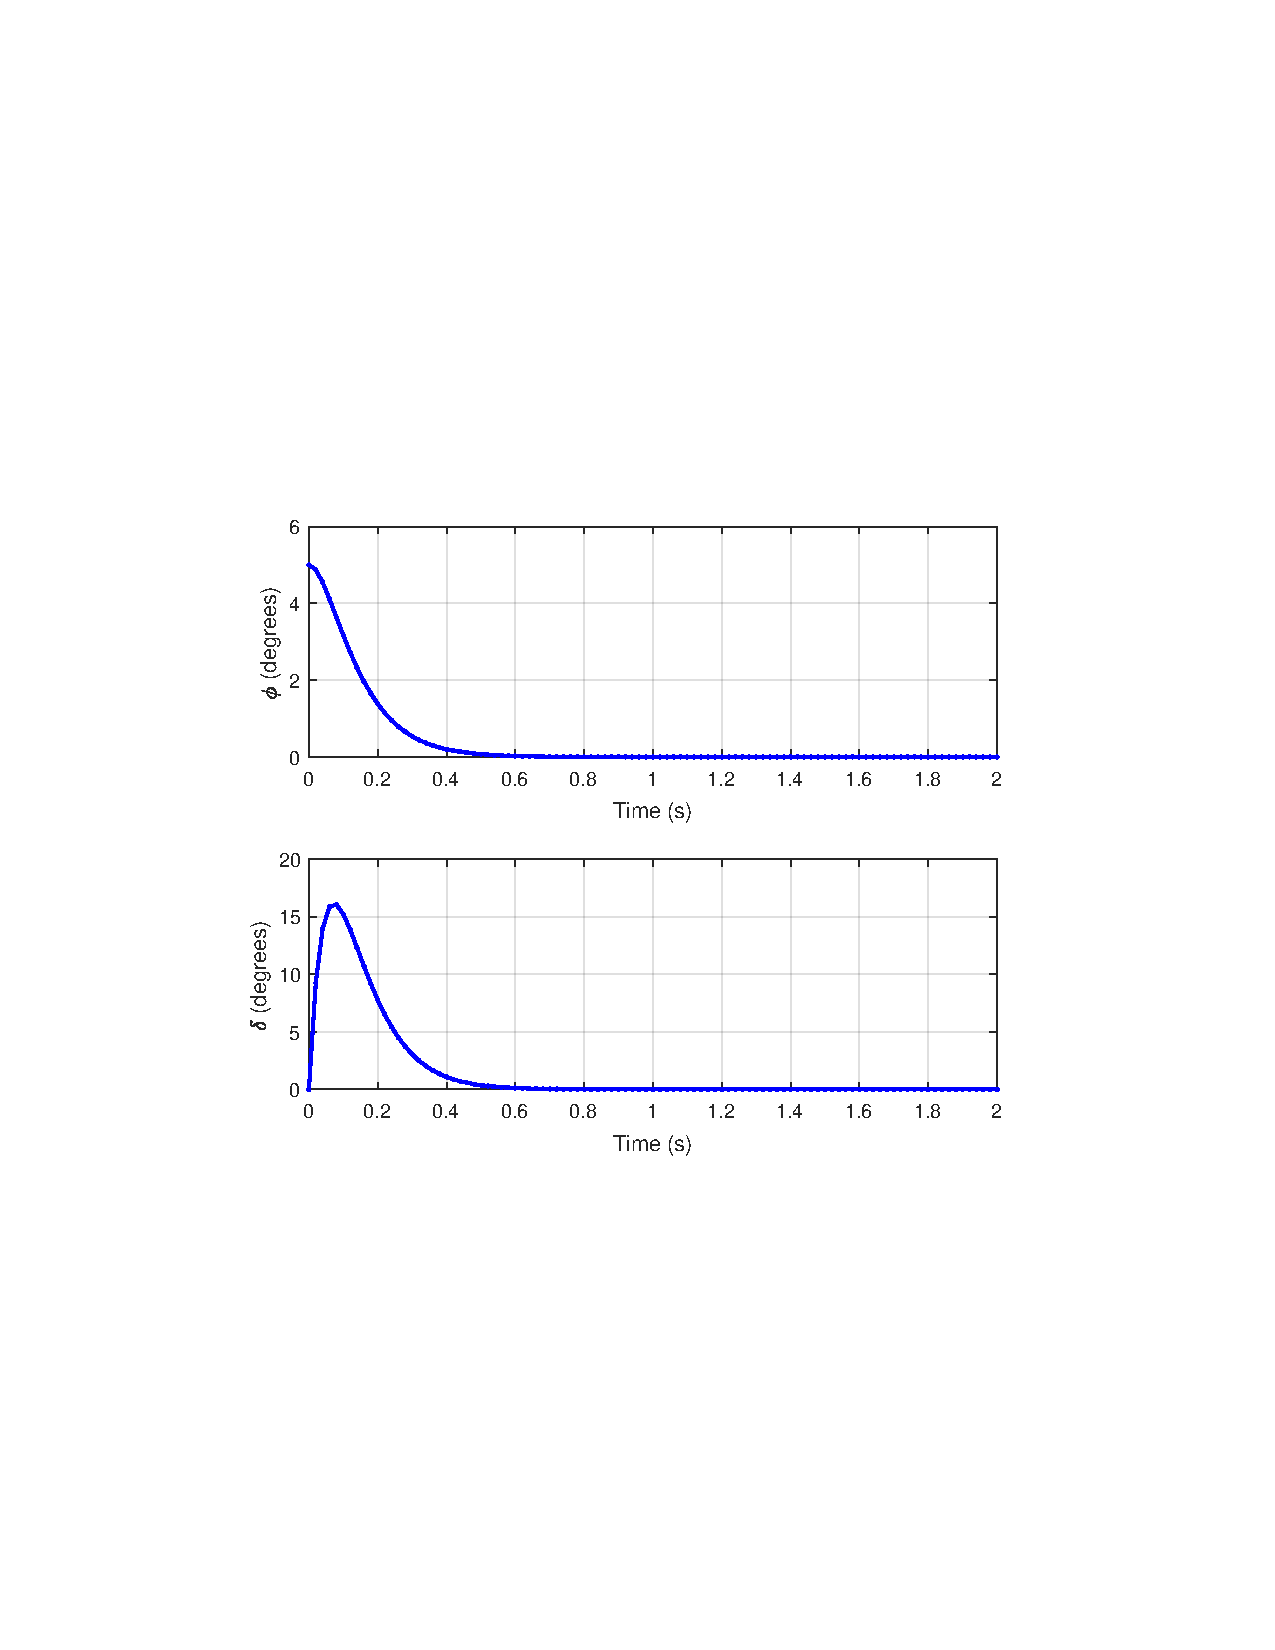
\includegraphics[width=\textwidth, trim=120 240 120 240]{figures/plots/LQR Compute Q(300,0,300)R(1) with no fork angle.pdf}
		\caption{\boldmath LQR with $Q = \operatorname{diag}(300,\,0,\,300)$, $R = 1$, $90^\circ$ fork angle.}
		\label{fig:lqr2}
	\end{subfigure}

	\vspace{0.5cm}

	\begin{subfigure}[b]{0.45\textwidth}
		\centering
		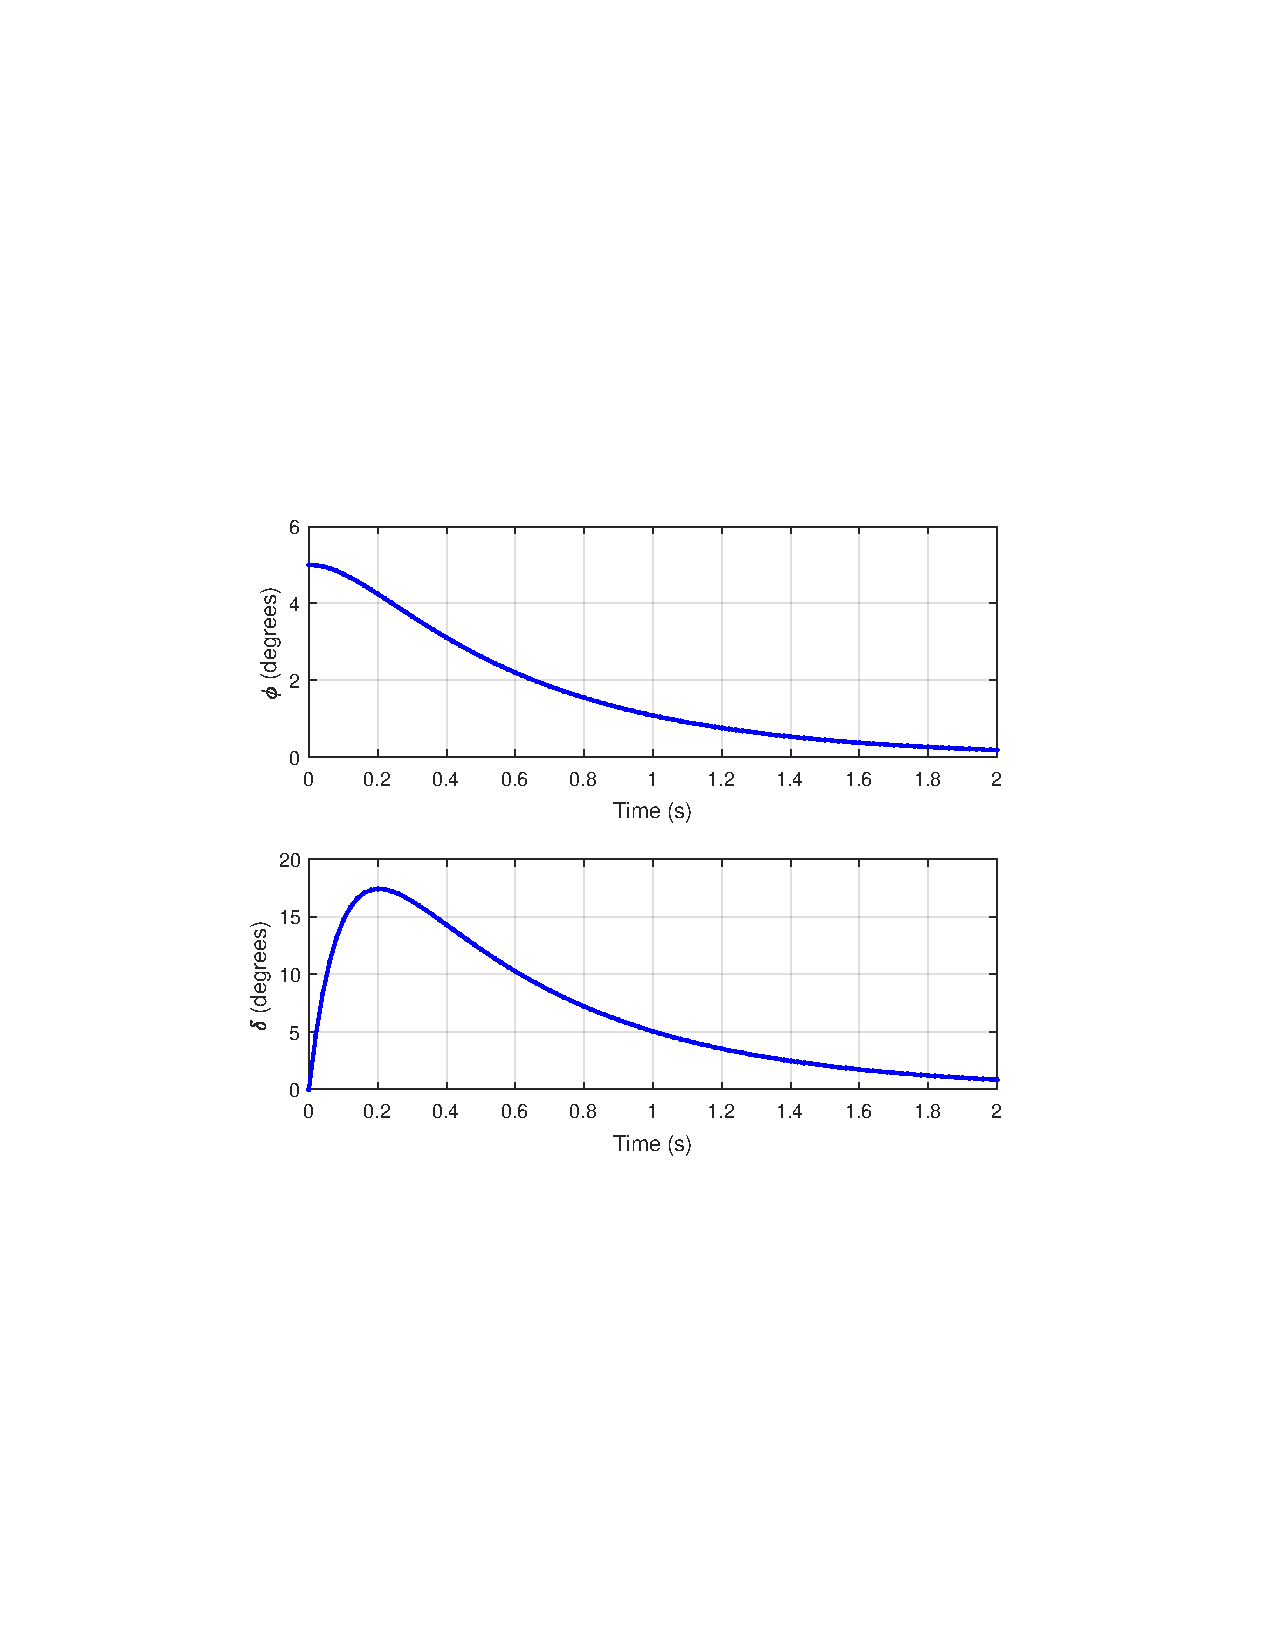
\includegraphics[width=\textwidth, trim=120 240 120 240]{figures/plots/LQR Compute Q(300,0,300)R(100) with no fork angle.pdf}
		\caption{\boldmath LQR with $Q = \operatorname{diag}(300,\,0,\,300)$, $R = 100$, $90^\circ$ fork angle.}
		\label{fig:lqr3}
	\end{subfigure}
	\hfill
	\begin{subfigure}[b]{0.45\textwidth}
		\centering
		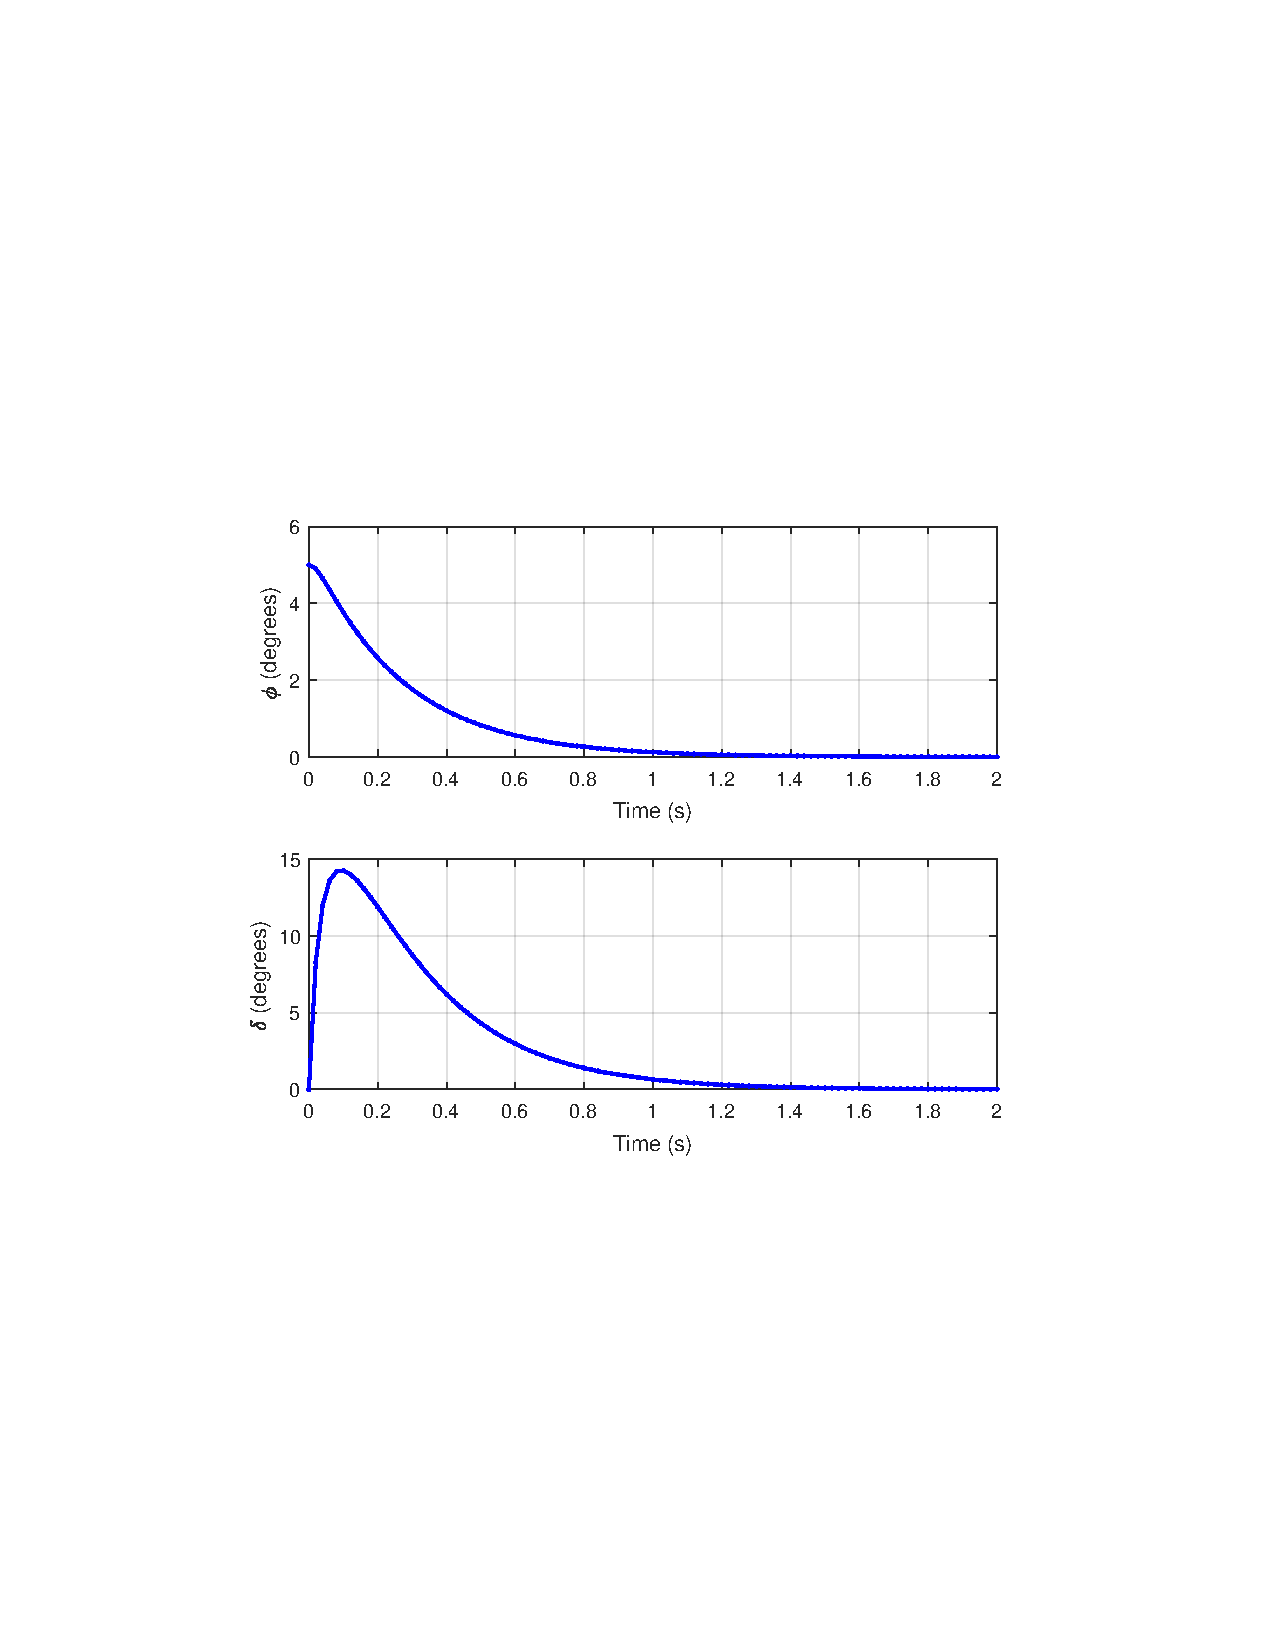
\includegraphics[width=\textwidth, trim=120 240 120 240]{figures/plots/LQR Compute Q(300,300,300)R(1) with no fork angle.pdf}
		\caption{\boldmath LQR with $Q = \operatorname{diag}(300,\,300,\,300)$, $R = 1$, $90^\circ$ fork angle.}
		\label{fig:lqr4}
	\end{subfigure}

	\caption{\boldmath Lean and steering angles over time under different LQR settings for an initial state vector (in radians) $x_0 = [0.0873, \, 0, \, 0]^\top$.}
	\label{fig:lqr_sim_figs}
\end{figure}

%%%%%%%%%%%%%%%%%%%%%%%%
\section{Data-Driven State-Feedback Controller}

Using input-state data, a data-driven state-feedback controller was constructed by solving a one-shot SDP problem mentioned in Equation \eqref{eq:final_gamma}.
This controller was obtained without knowledge of the exact system model, relying solely on the data and solving the optimisation problem.

This controller depends on obtaining input-state data. Therefore, a range of data was synthesised in simulation given an initial starting point for the system, an error bound for adding noise, and being controlled with a discrete LQR that stabilises the bicycle. The synthesised data formed a sequence where at each time step it was distorted with additive noise $\omega_i \in \mathbb{R}^n$ with independent components uniformly sampled as \[
\omega_i^j \sim \mathcal{U}\left[-\frac{\epsilon}{\sqrt{n}}, \frac{\epsilon}{\sqrt{n}}\right], \quad j = 1, \ldots, n,
\]
which can be compactly written as
\[
\omega_i \sim \mathcal{U}\left[-\frac{\epsilon}{\sqrt{n}}, \frac{\epsilon}{\sqrt{n}}\right]^n
\]
to satisfy  $\|\omega_i\|_\infty \leq \frac{\epsilon}{\sqrt{n}}$.

The data-driven state-feedback controller based on this data stabilised the bicycle efficiently and had similar or near coefficients to those of the discretised LQR.

Later, the output feedback gain vector from the LQR was applied on the real bicycle to collect some real data, instead of the synthesised data, for simulating and testing the data-driven state-feedback controllers. It turned out not to work since the process noise $\epsilon$ was too large for various segments of the data collected. From this, it was obvious that an online version of the data-driven state-feedback controllers would not work. This challenge is based on the real system errors compared to the synthesised data errors which were always bounded as needed.

In \autoref{fig:DDFBC_sim_figs}, the simulation results for different fork angles under identical settings are presented. The feedback gains are comparable to those obtained from the LQR controllers, demonstrating that the controller is capable of balancing the bicycle.

\begin{figure}[htbp]
	\centering
	\begin{subfigure}[b]{0.45\textwidth}
		\centering
		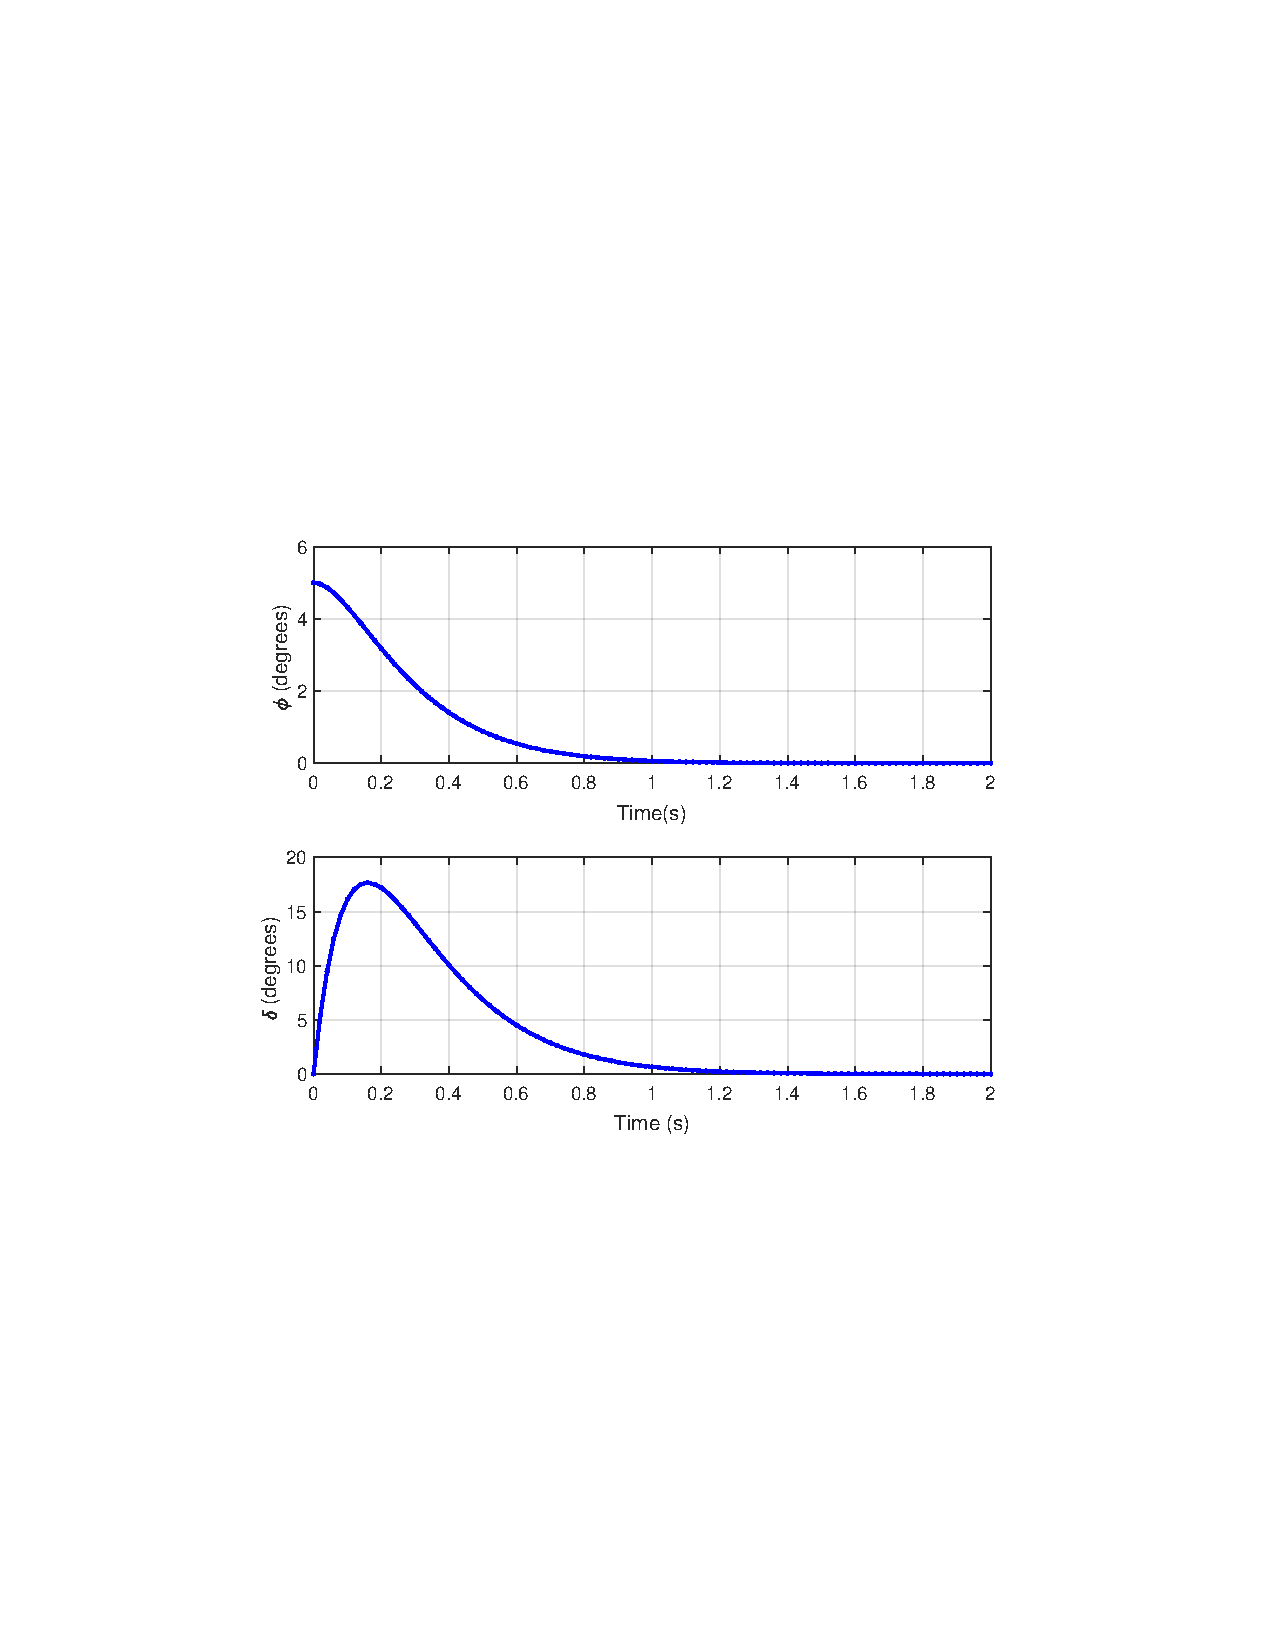
\includegraphics[width=\textwidth, trim=120 240 120 240]{figures/plots/DDSFB: Q(300,0.1,300)R(1) 75deg (-107.7 -12.75 6).pdf}
		\caption{\boldmath Data-driven state-feedback for $75^\circ$ fork angle.}
%		\label{fig:lqr1}
	\end{subfigure}
	\hfill
	\begin{subfigure}[b]{0.45\textwidth}
		\centering
		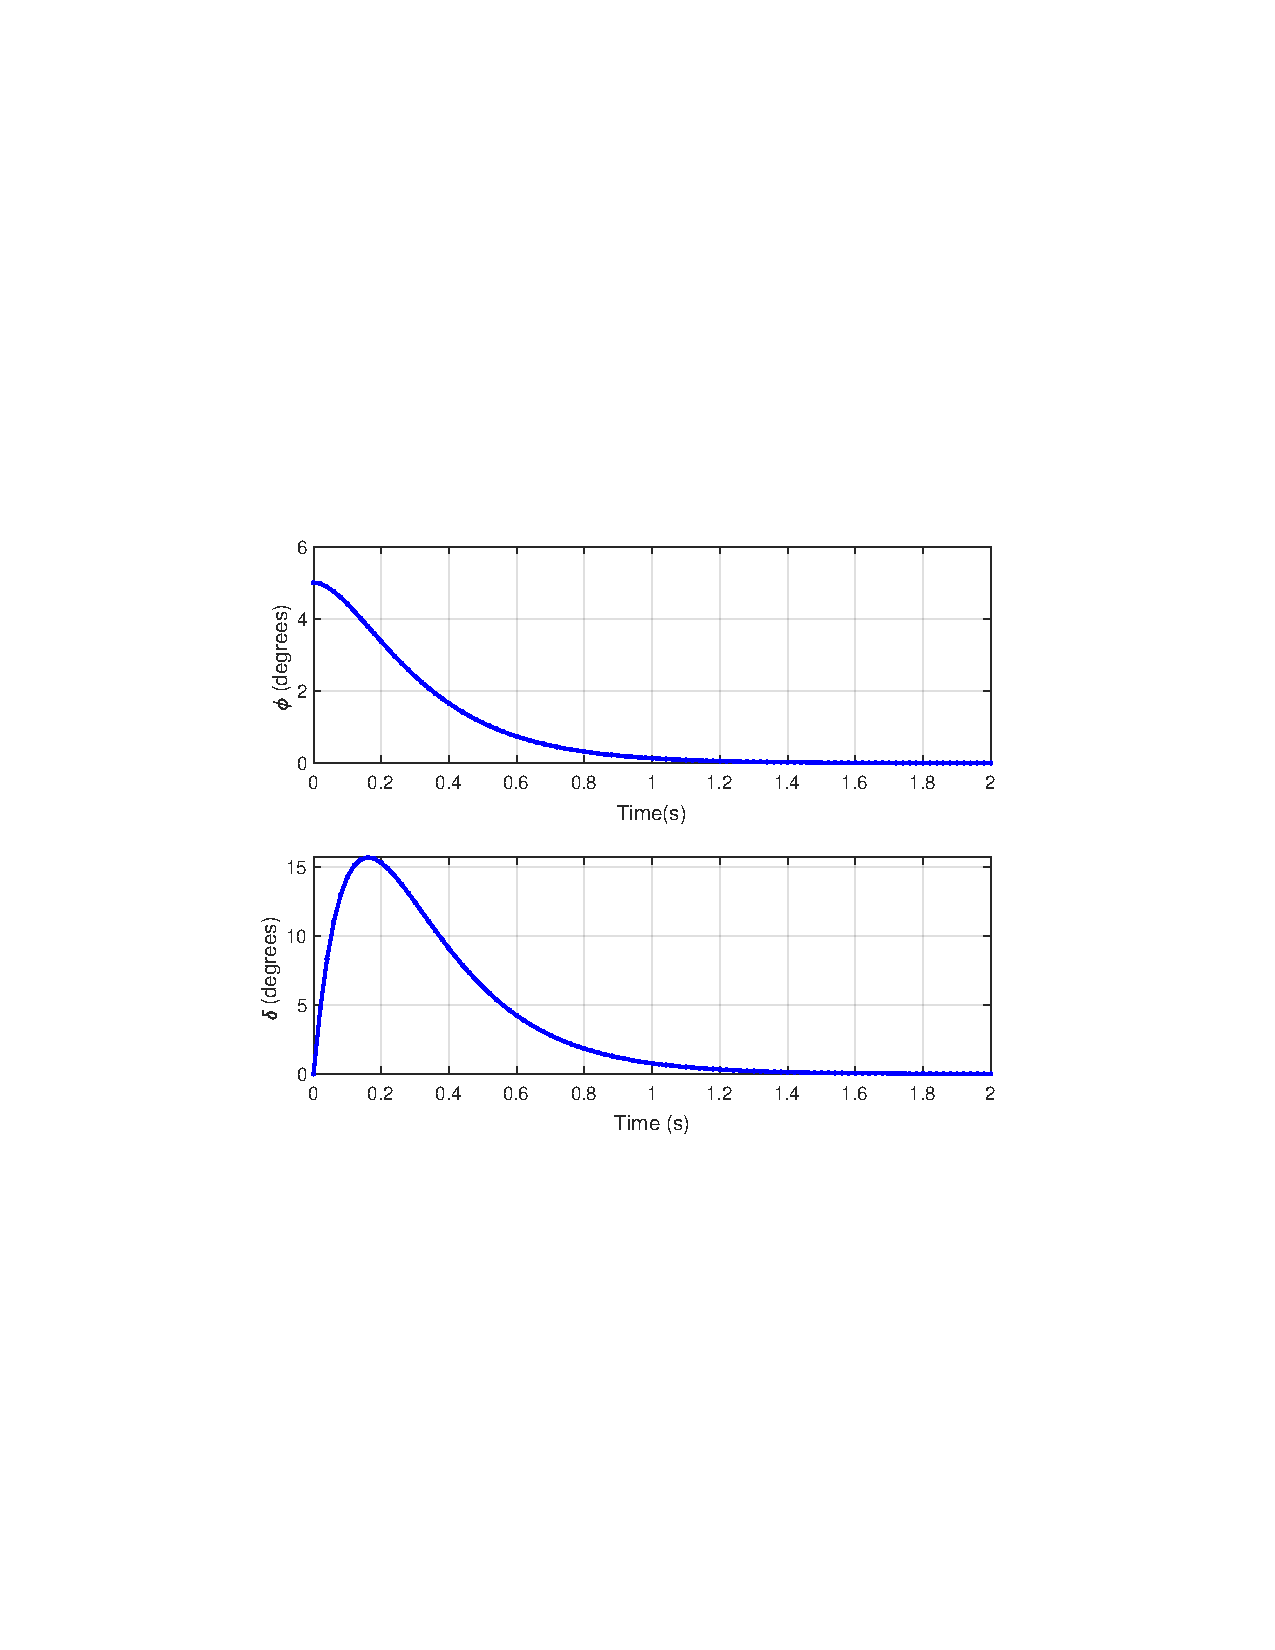
\includegraphics[width=\textwidth, trim=120 240 120 240]{figures/plots/DDSFB: Q(300,0.1,300)R(1) 90deg (-94.7 -9.7, 10.4).pdf}
		\caption{\boldmath Data-driven state-feedback for $90^\circ$ fork angle.}
%		\label{fig:lqr2}
	\end{subfigure}

	\caption{\boldmath Lean and steering angles over time under different data-driven state-feedback settings for an initial state vector (in radians) $x_0 = [0.0873, \, 0, \, 0]^\top$, $Q = \operatorname{diag}(300,\,0.1,\,300)$, $R = 1$, noise bound $\epsilon = 0.001$ and data length of $T = 40$.}
	\label{fig:DDFBC_sim_figs}
\end{figure}


%%%%%%%%%%%%%%%%%%%%%%%%
\section{Data-Driven Min-Max MPC Controller}

Finally, a full data-driven min-max MPC controller was implemented using synthesised input-state data similar to the previous controller.
Here, the SDP \eqref{eq:final_gamma} was solved in a receding horizon manner.

The simulation results for different fork angles under the same parameters are shown in \autoref{fig:DDMPC_sim_figs}.
The error bound $\epsilon$ is decreased to $10^{-5}$ to ensure obtaining a solution for the SDP at each iteration of the MPC.

\begin{figure}[htbp]
	\centering
	\begin{subfigure}[b]{0.45\textwidth}
		\centering
		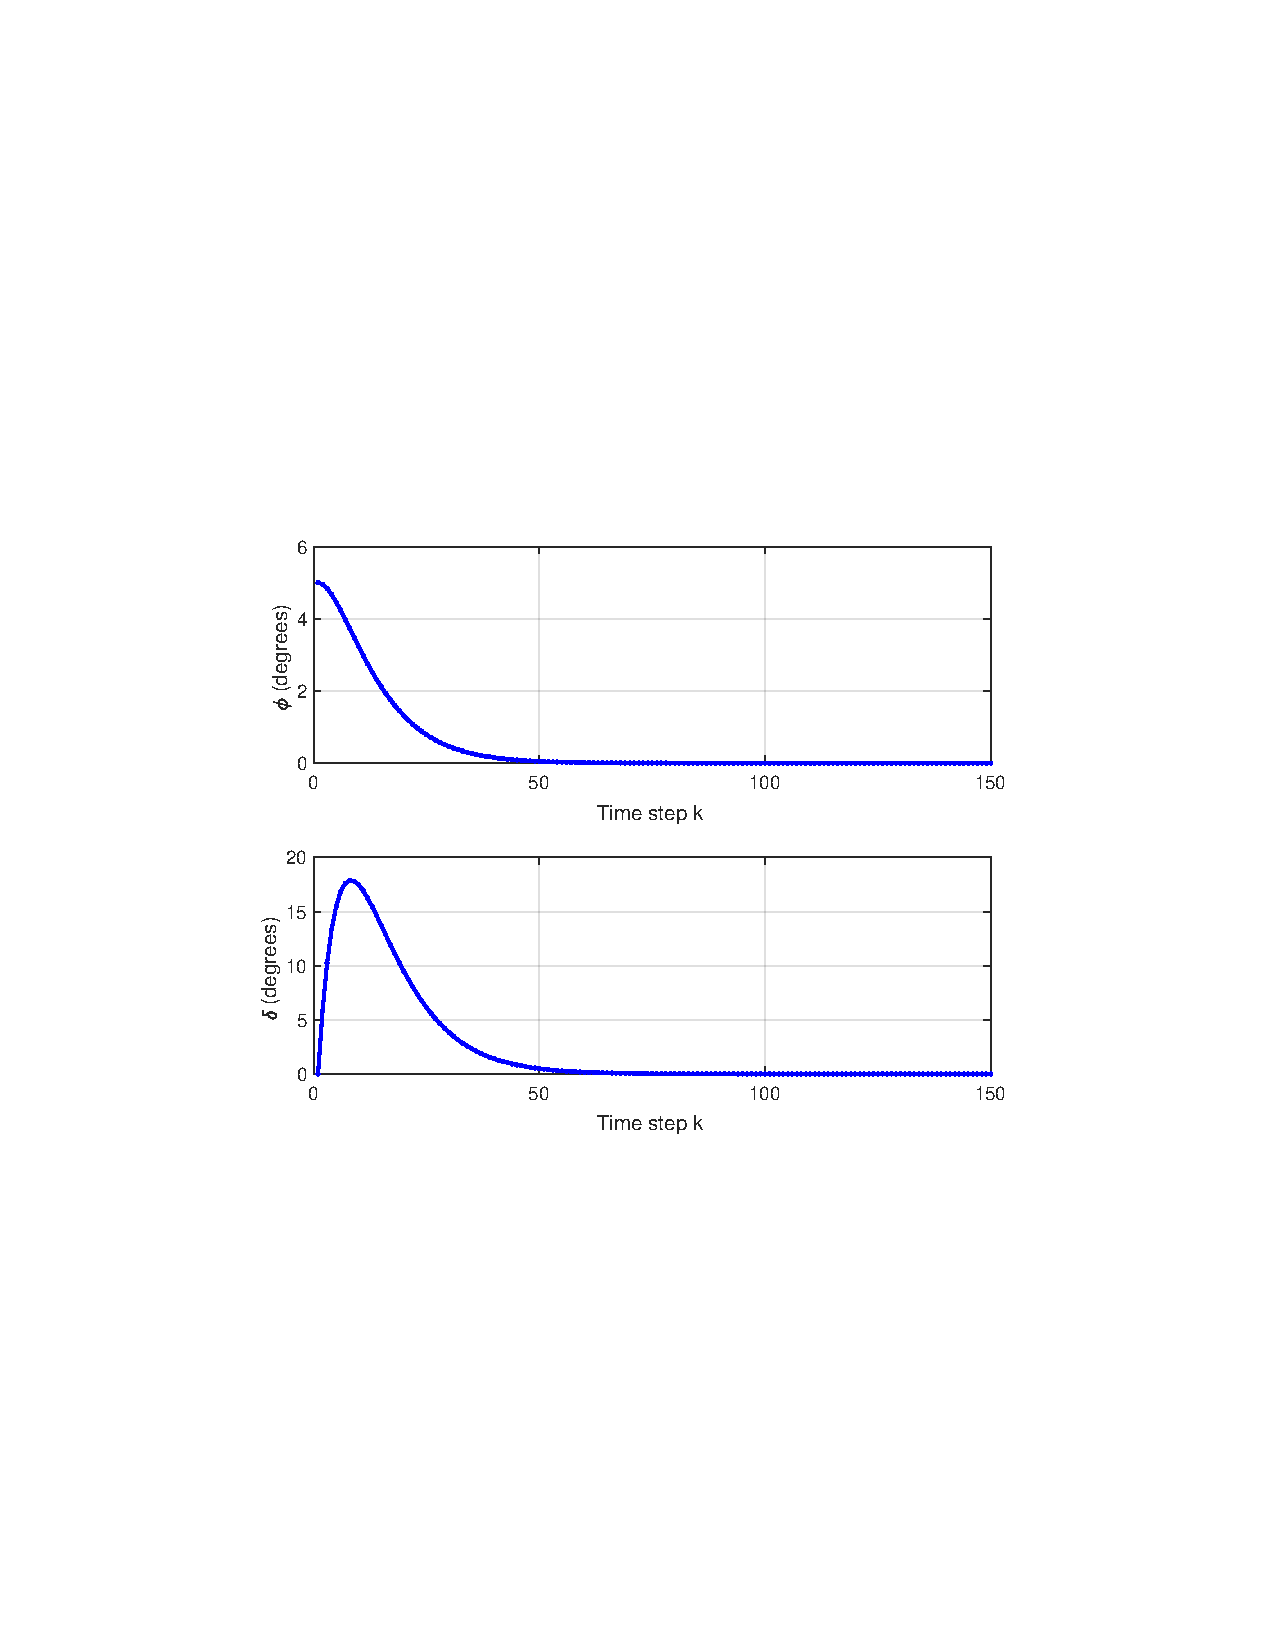
\includegraphics[width=\textwidth, trim=120 240 120 240]{figures/plots/DDMPC: Q(300,0.1,300)R(1) 75deg (-117, -11, 9).pdf}
		\caption{\boldmath Data-driven MPC for $75^\circ$ fork angle.}
		%		\label{fig:lqr1}
	\end{subfigure}
	\hfill
	\begin{subfigure}[b]{0.45\textwidth}
		\centering
		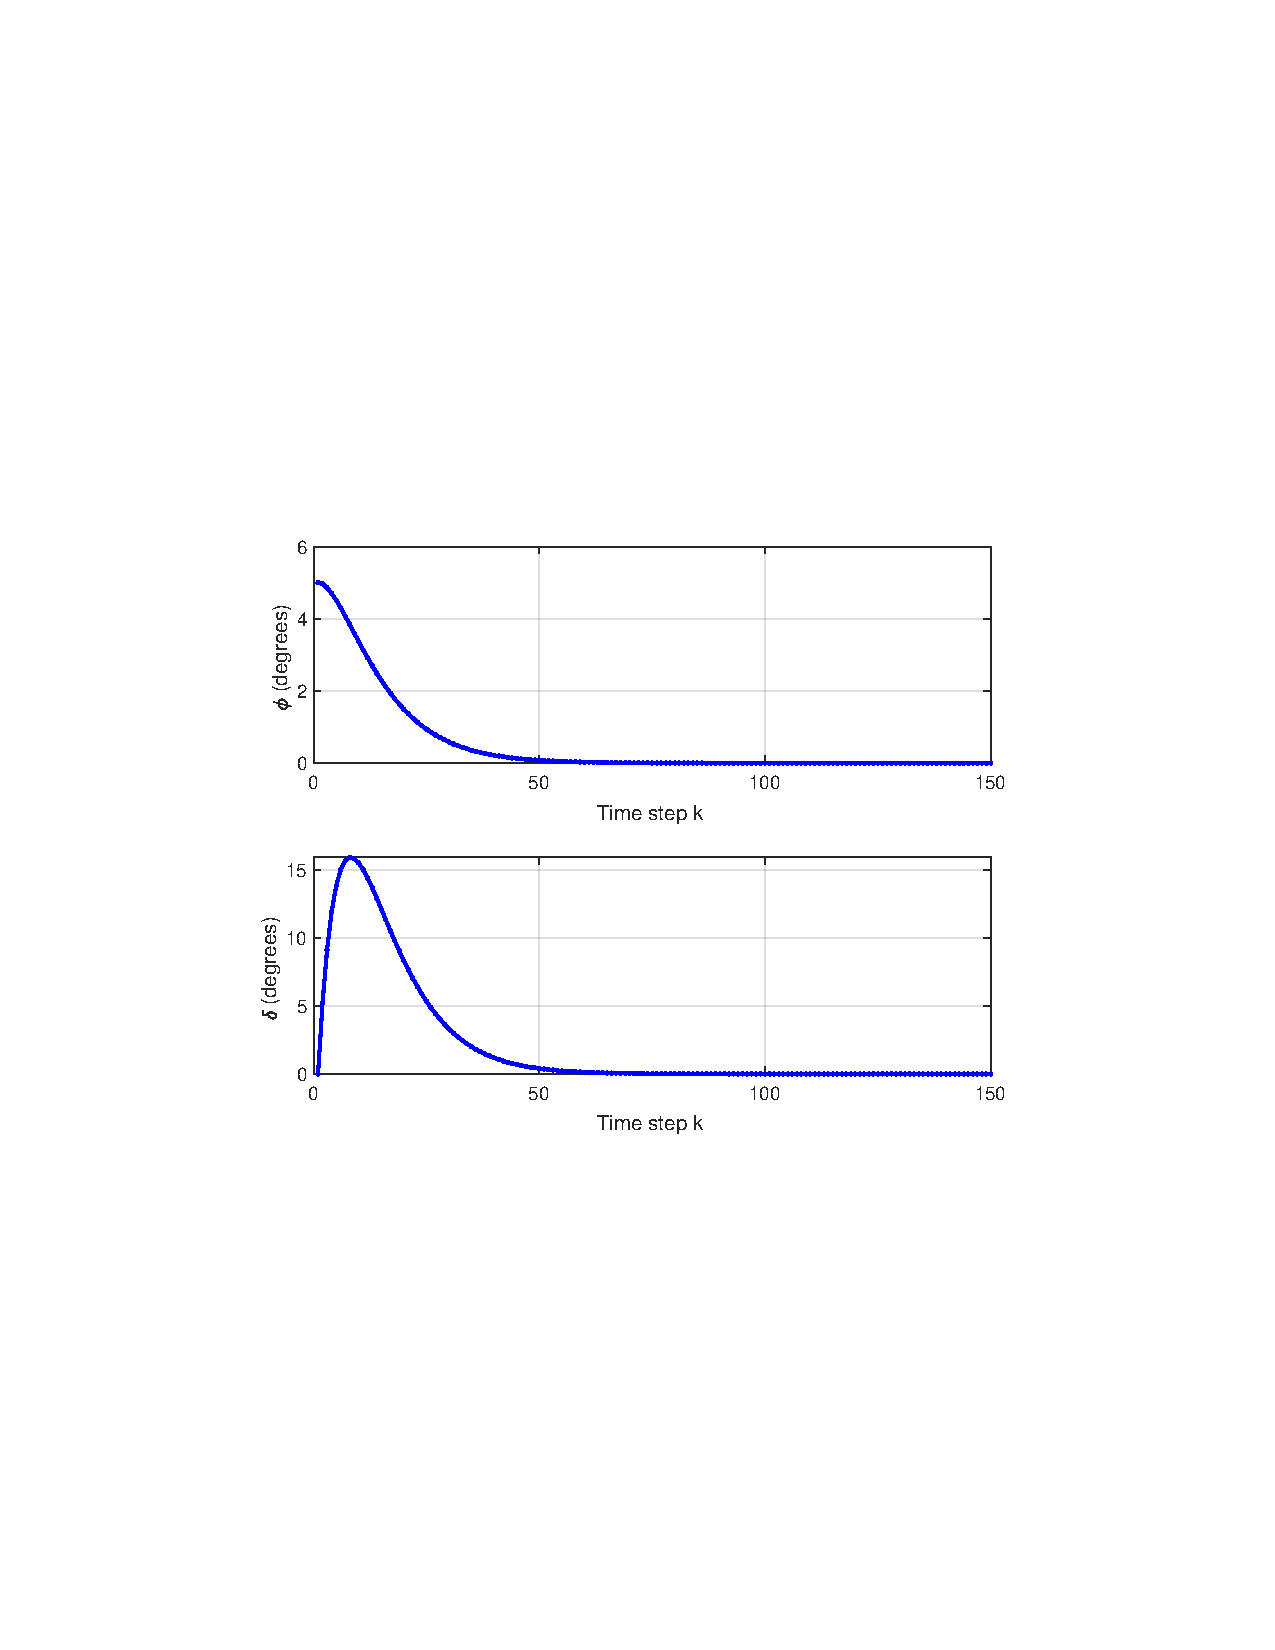
\includegraphics[width=\textwidth, trim=120 240 120 240]{figures/plots/DDMPC: Q(300,0.1,300)R(1) 90deg (-105, -9.87, 11).pdf}
		\caption{\boldmath Data-driven MPC for $90^\circ$ fork angle.}
		%		\label{fig:lqr2}
	\end{subfigure}

	\caption{\boldmath Lean and steering angles over time under different data-driven MPC settings for an initial state vector (in radians) $x_0 = [0.0873, \, 0, \, 0]^\top$, $Q = \operatorname{diag}(300,\,0.1,\,300)$, $R = 1$, noise bound $\epsilon = 10^{-5}$, data length of $T = 40$, and $mpc\_iterations = 150$.}
	\label{fig:DDMPC_sim_figs}
\end{figure}

\section{Comparisons?}
\todo[inline]{Add a Table for comparing costs here}

\improvement{Change this}{The simplified model, despite neglecting the fork geometry, proved more effective for fast controller design and practical implementation on resource-constrained platforms.}
This unexpected behaviour is probably resulting from the unknown parameters of the bicycle and interaction with the environment.

